
\section{Operating on the BST}

Operations include:

\begin{itemize}
  \item Efficient insertion and deletion.
  \item depth-first search by key
  \item forward and backwards traversal from any node.
  \item breadth-first search
  \item node presence
  \item delete node
  \item Search for node successor and predecessor
  \item Maximum and minimum queries.
\end{itemize}

Abstract data structures such as binary search trees support a standard
set of operations including insertion, deletion, search, etc. A closer look
at each of these operations follows.

\subsection{Least common ancestor}

The \textit{least common ancestor} (LCA) of two nodes $v$ and $w$ in a tree $T$ is the
lowest or deepest node which has $v$ and $w$ as descendants of itself, and where
each node is defined as a descendant of itself. The LCA is the shared ancestor located
farthest from the root of the tree $T$. Consider the following 3 node binary search tree.

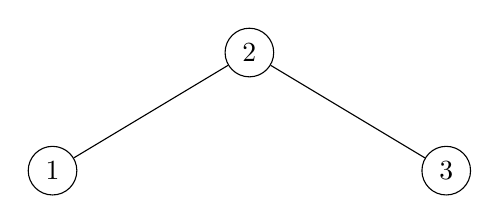
\begin{tikzpicture}[level/.style={sibling distance=50mm/#1}]
  \node [circle,draw] (z){$2$}
    child {node [circle,draw] (a) {$1$}}
    child {node [circle,draw] (j) {$3$}
  };
\end{tikzpicture}

We have the following cases:

\begin{enumerate}
  \item 1 is the LCA of 1.
  \item 2 is the LCA of 2.
  \item 3 is the LCA of 3.
  \item 2 is the LCA of 1 and 3.
  \item 2 is the LCA of 2 and 3.
  \item 2 is the LCA of 1 and 2.
\end{enumerate}

At least two algorithms may be employed to determine LCA. The first algorithm makes
two passes through $T$ to find a path from the root to the node. The second makes a
single pass through $T$, once down each branch. For the first algorithm, implementing
a path to node method is not difficult as it uses the same mechanics as the find method.

\lstset{language={Ruby}}
\begin{lstlisting}[frame=single,title=Two pass algorithm for LCA.]
def least_common_ancestor(key1, key2)
  (path(key1, []) & path(key2, [])).last
end

def path_to_node(key, collector)
  node = find(key) { |n| collector << n.key }
  raise KeyNotFoundError if node.nil?

  collector
end
\end{lstlisting}


\subsubsection{Error conditions}

The LCA algorithms fails if either node is not present in $T$. Handling this
condition is implementation dependent.


\subsection{Depth-first traverse}

\lstset{language={Ruby}}
\begin{lstlisting}[frame=single,title=Traverse the tree from the bottom up.]
def postorder_iterate
  return unless root

  current = find_unvisited_leaf_node root
  yield current

  while current.has_parent?
    current = find_unvisited_leaf_node current.parent
    yield current
  end
end
\end{lstlisting}

\lstset{language={Ruby}}
\begin{lstlisting}[frame=single,title=Find the deepest leftmost unvisited node relative to current.]
def find_unvisited_leaf_node current
  while current.has_unvisited_children?
    if current.left&.unvisited?
      current = current.left
    elsif current.right&.unvisited?
      current = current.right
    end
  end
  current.visit
end
\end{lstlisting}

\subsection{Successor and predecessor}

\setcounter{sno}{0}

\sno For an ordered list of values $x_i \in [x_0, x_1,\ldots,x_k]$, the successor of
$x_i$ is $x_{i+1}$, the predecessor $x_{i-1}$.

\sno Cormen et al.~\cite[p. 248-249]{cormen:th:1990} provide a succinct algorithm for
determining the successor given each node is linked to its parent.

\sno A decision has to made regarding the definition of minimum and maximum
elements in the tree. \sno The choices are having the relevant successor or
predecessors of such elements either be nil or be the node. \sno For this implementation,
maximum nodes are their own successors and minimum nodes are their
own predecessors.

\sno Here's an implementation in Python. \sno The nodes do not have a parent
pointer, so the parent must be passed along the recursion, along with
the correct predecessor.

\lstset{language={Python}}
\begin{lstlisting}[frame=single]
def get_predecessor(self, node, parent, predecessor):
    if parent.right == self:
        predecessor = parent

    if node.key == self.key:
        if self.left is not None:
            return self.left.minimum()
    else:
        return predecessor

    if node.key < self.key:
        if self.left is not None:
            return self.left.get_predecessor(node, self, predecessor)
    else:
        if self.right is not None:
            return self.right.get_predecessor(node, self, predecessor)

def predecessor(self, node):
    return get_predecessor(node, self, node)
\end{lstlisting}

\sno Implementing {\tt successor} is easy, use right for left, and find the
maximum where predecessor finds the minimum.

\subsection{Unvisit}

An \method{Unvisit} method needs to be implemented to ensure that once the
necessity for evaluating nodes for visited state has passed, all
the nodes in the tree can be reset to \attribute{visited = false}, allowing
future operations to proceed correctly. Implementation is easy,
simply pass a callback to any of the tree traversal functions which
sets \attribute{visited = false}.


\section{Properties of nodes}

Trees and nodes aren't the same thing, there is a logical separation.
That said, the behavior of the tree sometimes depends on the state of the
node.

\subsection{Visited and unvisited state}

When we visit a node during a walk or traverse of a tree, it might be
useful to mark whether the node has been visited. This is important, for
example, when performing depth-first searching, where the ``cursor'' has
to backtrack. The following methods help make the implementation easy
to understand:

\begin{itemize}
  \item \method{Visit} sets the node attribute \attribute{visited = true}.
  \item \method{Is\_Visited} (or \method{Visited?}) replies with the boolean
    state of the node, true when the \attribute{visited} is set.
  \item \method{Is\_Unvisited} (or \method{Unvisited?} is the default state
      of each node.
\end{itemize}

\subsubsection{Test cases for \method{Visited?} and \method{Unvisited?}}

Testing is almost superfluous. For TDD, the tests can be set up
to verify that setting and unsetting the visited state is correctly
performed. Later, these tests could be removed and the visited and
unvisited helper methods moved to private methods.

\subsection{\method{has\_unvisited\_children?}}

\lstset{language={Ruby}}
\begin{lstlisting}[frame=single,title=Helper methods for determining child's status.]
def unvisited?
  !visited
end

def has_unvisited_children?
  return false unless has_children?
  left&.unvisited? || right&.unvisited? ? true : false
end
\end{lstlisting}

\section{Breadth-first traversal}

Breadth-first traveral can be used for searching, for determining whether a key exists,
or for writing out the tree in flat format with rows and pointers.

For persistence, we have the following:

\begin{itemize}
\item At each node we can store pointers to each child.
\item We can store the start and the stop of each row separately.
\item We can store an array of arrays, where each of the arrays is
      one level of the tree.
\end{itemize}

[
 [root],
 [ root.left, root.right],
 [...]
]

Can all the pointers be stored in one pass, then process in a second pass,
or can the nodes be processes as the breadth-first traverse proceeds?

